\documentclass[12pt]{article}
\usepackage{amssymb, amsmath, amsfonts, bm, graphicx, geometry,cancel}
\usepackage{tabularx, booktabs, float, enumitem, multicol, mathtools}
\geometry{margin=1in}


\title{}
\date{}
\author{}

\begin{document}
\section*{Introduction}
The first half of the semester, consisting of Units 1–3, is an application of classical physics to understand the behavior of light. Starting with Unit 4, we begin to explore experiments that classical physics cannot explain, leading us to develop new models based on quantum mechanics. In Unit 4, we explore experimental results that suggest there are limitations with classical physics, and in Unit 5, we formalize quantum mechanics to explain these results.\\

{\centering\LARGE Unit 4: Modern Physics\par}\noindent
In this unit, we explore the failures of classical explanations for certain experimental phenomena, which will lead to the development of a \textit{quantized} model of modern physics. We will begin with the development of the atomic model.\\\\
Generally, classical physics refers to the fields of Newtonian mechanics, electromagnetism, and thermodynamics.
\section*{Evolution of Atomic Models}
\textbf{1800: Invention of the First Battery}\\
When Alessandro Volta invented the first battery, electricity was thought to be a fluid that flowed through wires.\\\\
As a result of this discovery, scientists were able to perform \textit{electrolysis}. By passing electricity through water, they were able to prove that water was made of two different elements, hydrogen and oxygen. Previously, water was thought to be basic and indivisible.\\\\
\textbf{1808: Dalton Model}\\
John Dalton argued that all matter is made up of atoms, which are indivisible and indestructible.\\\\
\textbf{1820: Cathode Ray}\\
When Michael Faraday tried to pass electricity through a gas, he observed that the current splits the gas into positively and negatively charged ions. The negative discharge always had a green glow, called a \textit{cathode ray}.
\begin{center}
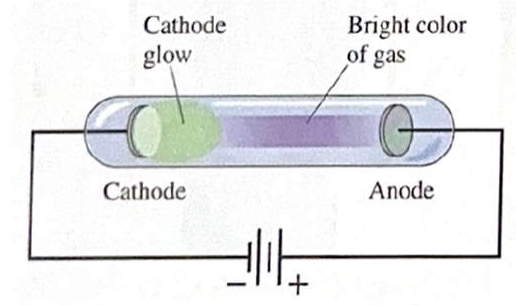
\includegraphics[width=0.4\textwidth]{Cathode Ray.png}
\end{center}
This proved that atoms were not indivisible, as they could be split into charged particles.\\\\
\textbf{1888: Discovery of the Electron}\\
J.J. Thomson discovered the electron by applying a magnetic field to the cathode ray. He observed that the cathode ray was deflected by the magnetic field, which suggested that it was made of negatively charged particles.
\begin{center}
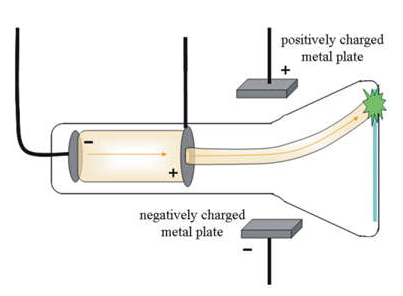
\includegraphics[width=0.6\textwidth]{CRT.png}
\end{center}
Thomson then proposes the \textbf{plum pudding atomic model}. That atoms are composed of \textit{discrete} negatively charged electrons in a \textit{continuous} positively charged medium.\\\\
\textbf{1905: Miliken's Oil Drop Experiment}\\
Robert Miliken finds that the charge on each varying oil drop is a multiple of $1.6 \times 10^{-19}$ C. Thus, he proposes that the \textbf{charge of an electron} is $e=1.6 \times 10^{-19}$ C.\\\\
Here, we realize that \textit{charge is quantized}: $q = ne$, where $n=\pm 1, \pm 2, \pm 3, \ldots$.
\begin{center}
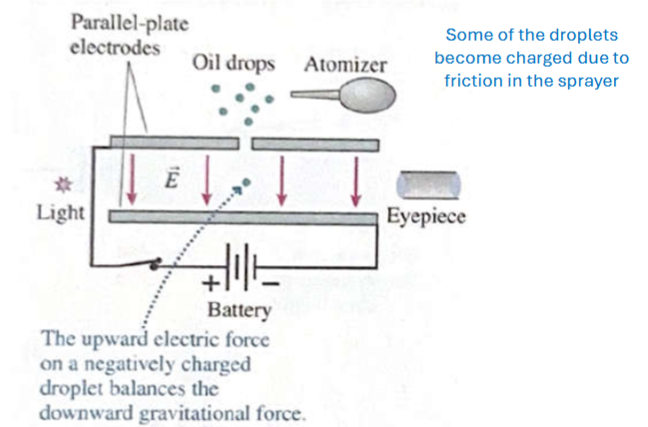
\includegraphics[width=0.6\textwidth]{miliken.png}
\end{center}
\newpage\noindent
\textbf{1909: Gold Foil Experiment}\\
Ernest Rutherford finds that the atoms are mostly empty space with a small, dense, positively charged nucleus. Thus, he proposes the \textbf{Rutherford atomic model}, where electrons orbit a small, dense positively charged nucleus.
\begin{center}
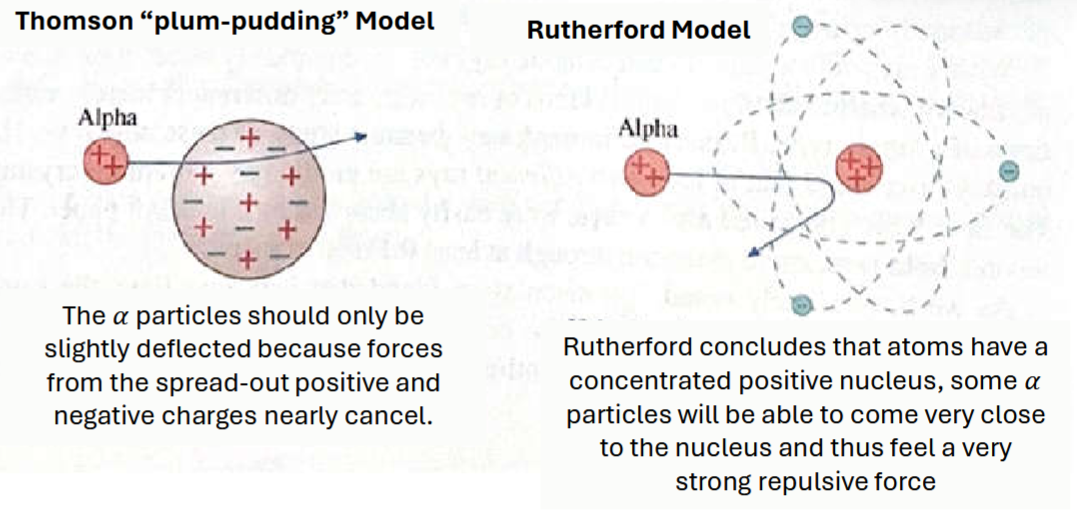
\includegraphics[width=0.8\textwidth]{Rutherford.png}
\end{center}
\textbf{1913: Bohr Model}\\
It would not be until Niels Bohr that we would have a quantized model of the atom. Bohr's atom is based on the Rutherford model, but with the addition of quantized energy levels.\\\\
\textbf{1926: Schrodinger Model}\\
Finally, Erwin Schrodinger develops the quantum mechanical model of the atom, which explains the quantized nature of the atom using quantum mechanics. Instead of discrete electrons orbiting the nucleus, Schrodinger's model describes electrons as a \textit{cloud} of probability around the nucleus.\\\\
Generally, this development shows an intuition that we need to apply to our current understanding of classical physics to develop modern physics that explains the quantized nature of the universe. In the atomic model, we see through a series of experiments that classical assumptions of continuous charge and energy were incorrect. We will then continue this intuition through the discrete emission spectrum of hydrogen, which classical models of continuous light could not explain.
\section*{Emission and Absorption Spectra}
We find that different elements emit and absorb light at discrete wavelengths. The \textbf{absorption spectrum} describes the wavelengths of light that are not reflected by an element after being exposed to a continuous spectrum of light. The \textbf{emission spectrum} describes the wavelengths of light that are emitted by an element after being excited by an external energy source.
\begin{center}
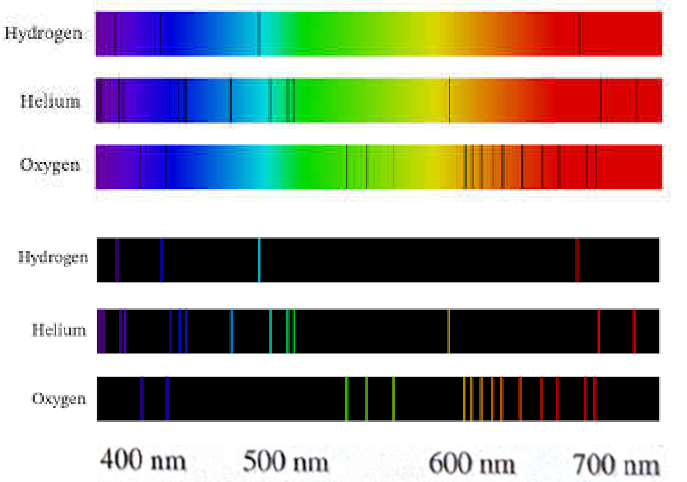
\includegraphics[width=0.6\textwidth]{spectrum.png}
\end{center}
\textbf{Rydberg Formula}\\
\textit{Experimentally derived}, the Rydberg formula describes the wavelengths of light \underline{emitted by Hydrogen}.
\[\boxed{\frac{1}{\lambda} = R_H \left( \frac{1}{m^2} - \frac{1}{n^2} \right),\quad R_H \approx 1.097 \times 10^7 \, \text{m}^{-1}}\]
For integers $n>m$ where $m$ is the higher energy level and $n$ is the lower energy level.
\begin{center}
\begin{tabular}{c l l}
\hline
$m$ & Series Name & Region \\
\hline
1 & Lyman     & Ultraviolet \\
2 & Balmer    & Visible \\
3 & Paschen   & Infrared \\
4 & Brackett  & Infrared \\
5 & Pfund     & Infrared \\
6 & Humphreys & Infrared \\
$7+$ & ---     & Infrared / Microwave \\
\hline
\end{tabular}
\end{center}
\underline{Note:} For transitions between energy levels, emission occurs when an electron moves from a higher level to a lower one ($n \to m$), while absorption occurs when it moves from a lower level to a higher one ($m \to n$).\\\\
Electrons \textit{emit} a photon when dropping energy levels and \textit{absorb} a photon when gaining energy levels. Since they emit and absorb light, we can relate frequency to wavelength using the speed of light: 
\[\boxed{c = \lambda f}\] 
\newpage
\section*{Blackbody Radiation}
Blackbody radiation is another example of a where classical models fail to match experimental results. Notably, we will see that the classical model of blackbody radiation, the Rayleigh-Jeans law, predicts an infinite amount of energy emitted at short wavelengths (high frequencies), which is known as the \textit{ultraviolet catastrophe}.\\\\
\textbf{Thermal Radiation}\\
Unlike individual elements, most solids and liquids emit and absorb a continuous spectrum of radiation called \textbf{thermal radiation}, which depends on the temperature of the object. However, thermal radiation is typically not in the visible range, which is why most visible light we see from objects is reflected light. Colors result from the wavelengths of light that are reflected by an object, while the rest are absorbed.
\begin{center}
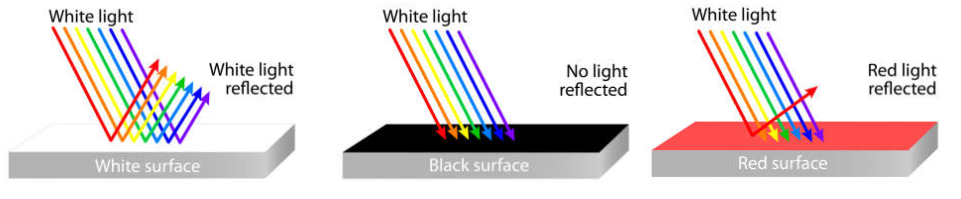
\includegraphics[width=1\textwidth]{reflection.png}
\end{center}
At sufficiently high temperatures, an object begins to emit visible light as well. For example, glowing hot metal and incandescent light bulbs emit visible light due to their high temperatures.\\\\
\textbf{Blackbody Radiation (Ideal Model)}\\
To study thermal radiation without having to account for the reflected light from an object, we use the idealized model of a \textbf{blackbody}, which is an object that perfectly absorbs all incident light (zero reflection) and emits thermal radiation based on its temperature.
\begin{center}
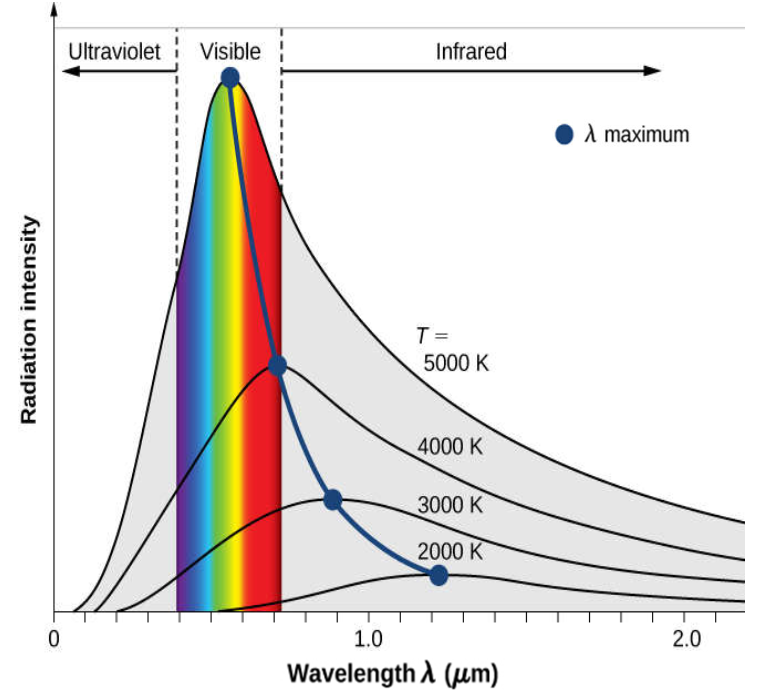
\includegraphics[width=0.5\textwidth]{blackbody.png}
\end{center}
Because thermal radiation is dependent only on temperature, blackbodies at the \textit{same temperature} all emit the same continuous spectrum of light, regardless of their material.\\\\
Stefan-Boltzmann finds that increasing the temperature of a blackbody increases the \textit{intensity of all wavelengths emitted}. This is described by the \textbf{Stefan-Boltzmann Law}, which was found experimentally, that describes the intensity of radiation emitted by a blackbody at a given temperature:
\[\boxed{\frac{P}{A} = \sigma T^4, \quad \sigma=5.67 \times 10^{-8} \,\frac{\text{W}}{\text{m}^2 \cdot \text{K}^4}}\]
Where $\sigma$ is the Stefan-Boltzmann constant, $P$ is the power emitted by the blackbody, and $A$ is the surface area of the blackbody.\\\\
\underline{Note:} Intensity is defined as the power per unit area, which is the amount of energy emitted per second per square meter.\\\\
Additionally, the spectrum shifts towards shorter wavelengths (higher frequencies) as the temperature increases.
This is described by \textbf{Wein's Law}, which was found experimentally, that describes the wavelength of peak intensity at a given temperature:
\[\boxed{\lambda_\text{peak} = \frac{[2.90\times10^6\,\text{nm}\cdot\text{K}]}{T}}\]
\underline{Note:} Use kelvin for temperature! ($K = ^\circ C + 273.15$)\\\\
Notably, the Sun is a blackbody that has the perfect temperature to emit its peak intensity in the visible range, which is why we see a continuous visible spectrum of light from the Sun.
\section*{Rayleigh-Jean Model (Classical Model)}
\underline{\textbf{Note (New notation)}}: $\nu$ denotes frequency, replacing the earlier use of $f$.\\\\
Classically, we can model a blackbody as a cavity with perfectly reflecting walls and a small window.
\begin{center}
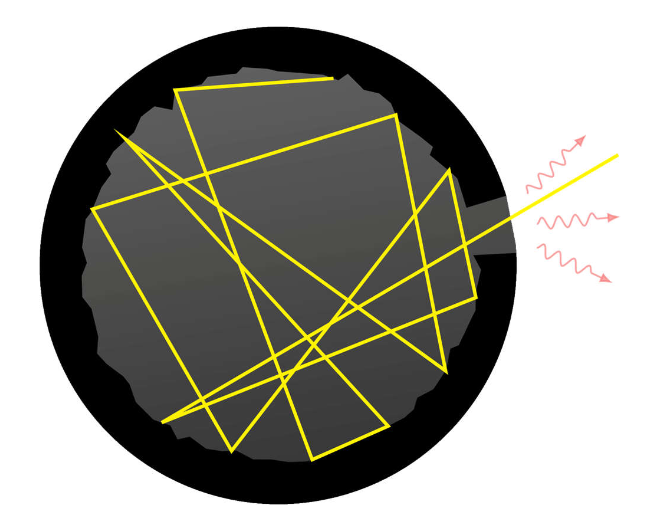
\includegraphics[width=0.4\textwidth]{classical blackbody.png}
\end{center}
Any light incident on the window it will be bounced around the reflective walls so many times that it will eventually be absorbed before it can exit the window (perfect absorption). As the walls absorb the kinetic energy of the light, it will increase in temperature.\\\\
As temperature (averaged out kinetic energy) increases to a high enough level, charges within the walls will begin to accelerate and emit light. Thus, the blackbody will emit thermal radiation.\\\\
The Rayleigh-Jean model is based on the idea that the "trapped" light inside the cavity exists as 3D standing electromagnetic waves (all trapped waves must have nodes at the walls). We can model the number of \textit{modes per unit volume} ($N(\nu)$) of the trapped light as a function of frequency $\nu$:
\[N(\nu) = \frac{8\pi \nu^2}{c^3}\]
A mode refers the specific standing wave pattern that exists at a given frequency within the cavity. Because higher frequencies have shorter wavelengths, there area greater number of mode combinations ($n_x, n_y, n_z$) that can fit within the cavity, compared to lower frequencies.\\\\
Finally, we assign energy to each mode of the trapped light based on the equipartition theorem, giving it an average energy of $\langle E \rangle = k_B T$ per mode, where $k_B$ is the Boltzmann constant.\\\\
Thus, the \textbf{Rayleigh-Jean model} relates the energy density ($u_T(\nu)$) contained per unit volume of the radiation within the cavity at a given frequency $\nu$ and temperature $T$ as:
\[\boxed{u_T(\nu) = \langle E \rangle N(\nu)  = \frac{8\pi \nu^2 k_B T}{c^3},\quad k_B = 1.3806 \times 10^{-23} \,\frac{\text{J}}{\text{K}} }\]
\textbf{Problems with the classical model:}
\begin{center}
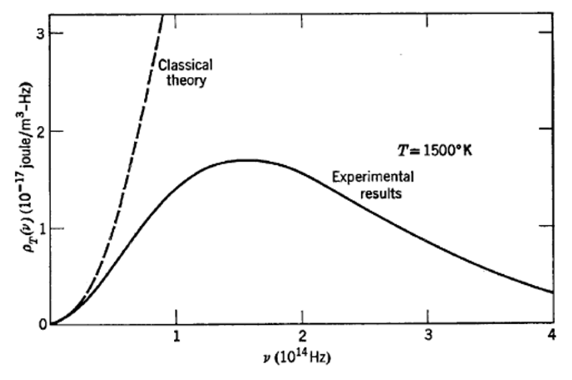
\includegraphics[width=0.6\textwidth]{Rayleigh Jean.png}
\end{center}
\begin{itemize}
    \item UV Catastrophe: The energy density goes to infinity as frequency increases, which deviates from experimental results.
    \item Infinite total energy: The total energy density across all frequencies should be finite but the Rayleigh-Jean model predicts an infinite total energy density emitted by the blackbody.
    \[U(T) = \int_0^\infty u_T(\nu) d\nu\]
\end{itemize}
These problems are the result of our assumptions that the atoms within the wall can absorb and emit a continuous range of energies (it is actually discrete), and that every mode of oscillation is equally likely to be excited (it is actually less likely for higher frequencies).
\section*{Planck's Model (Quantized Model)}
To address the inaccurate assumptions of the Rayleigh-Jean model, Max Planck proposed a new model of blackbody radiation that incorporates the idea of quantization.\\\\
He suggests that the oscillators in the walls of the cavity can only absorb and emit \textit{discrete} packets of energy, which he called quanta. He then proposes that oscillators of frequency $\nu$ can only absorb quanta of energy \textit{proportional to} $\nu$:
\[E_n = n h \nu, \quad n = 1, 2, 3, \ldots\]
Where $h=6.626 \times 10^{-34} \,\text{J}\cdot\text{s}$ is the \textbf{Planck constant}.\\\\
This way, exciting higher frequency modes will require more energy, which is less likely to occur at a given temperature. Thus, instead of assigning an equal average energy, Planck finds:
\[\langle E \rangle = \frac{h\nu }{\exp{\left(\frac{h\nu}{k_B T}\right)}-1}\]
\textbf{Planck's model} then states:
\[\boxed{u_T(\nu) = \frac{8\pi h}{c^3} \frac{\nu^3}{\exp{\left(\frac{h\nu}{k_B T}\right)}-1}}\]
This agrees with experimental results and matches the Rayleigh-Jean model at low frequencies. Additionally, the total energy per unit volume is finite:
\[U(T) = \frac{8\pi h}{c^3} \int_{0}^{\infty}  \frac{\nu^3}{e^{\frac{h\nu}{kT}} - 1}\, d\nu = aT^4\]
Here, we obtain a huge idea: the fact that energy is quantized. This same intuition will be applied to the atomic model, where we will see that elements emit and absorb light at discrete wavelengths because electrons can only exist at discrete energy levels.\\\\
Albert Einstein will apply this idea of quanta to light itself in the photoelectric effect, introducing the concept of photons, which are quanta of light.
\newpage
\section*{Photoelectric Effect}
Experimentally, in 1902, Lenard established the following relationships between light incident on a metal surface and the photoelectrons emitted from that surface:
\begin{itemize}
\item Photoelectrons are only emitted if the frequency of the incident light is above a certain threshold frequency ($\nu_0$) that is specific to the metal. 
\item Increasing the \textit{intensity} of the incident light increases the number of photoelectrons emitted but does not affect their kinetic energy.
\item Increasing the \textit{frequency} of the incident light increases the kinetic energy (speed) of the emitted photoelectrons but does not affect the number of photoelectrons emitted.
\end{itemize}
In 1905, Einstein applies the idea of quantization to light, proposing that light is not a continuous wave but rather discrete packets of energy called \textbf{photons}. Each photon has an energy proportional to its frequency:
\[\boxed{E_\text{photon} = h\nu}\]
Since photons have quantized energy, they can only be absorbed by a material in integer values (it must absorb a whole photon, not a fraction of a photon). Additionally, when a substance absorbs a photon, all the photon's energy goes to \textit{one electron}, raising its energy level.
\begin{center}
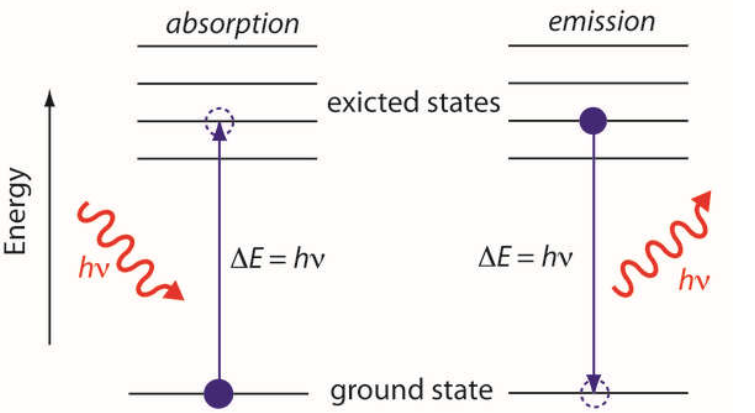
\includegraphics[width=0.6\textwidth]{photon.png}
\end{center}
\textbf{Photoelectric Effect}\\
The photoelectric effect describes the emission (release) of electrons from a material when it absorbs photons. Thus, we describe the \textit{minimum energy} required to emit a photoelectron as the \textbf{work function} ($W$) of the material.
\[\boxed{W=h\nu_0}\]
Where $\nu_0$ is the threshold frequency of the material and is dependent on the material's properties.\\\\
If the energy of the incident photon ($E_\text{photon} = h\nu$) is greater than the work function, then the excess energy will be converted into kinetic energy of the emitted photoelectron:
\[\boxed{K_\text{max} = h\nu-W}\]
\begin{center}
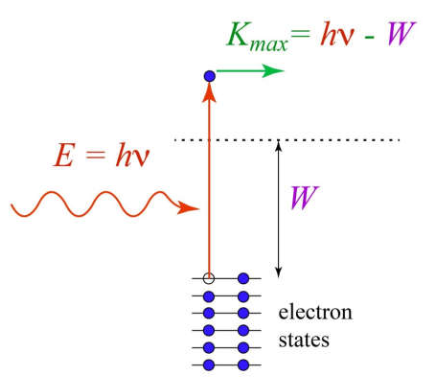
\includegraphics[width=0.4\textwidth]{Photoelectric.png}
\end{center}
Thus, staying consistent with experimental findings:
\begin{itemize}
    \item Incident light with higher intensity $\implies$ more incident photons and thus more photoelectrons emitted.
    \item Incident light with higher frequency $\implies$ higher $E_\text{photon}$ and thus higher kinetic energy of emitted photoelectrons.
\end{itemize}
\textbf{Electron Energy Transitions}\\
This theory of quantized energy (photons) can also be applied to the raising and lowering of electrons between energy levels in an atom.
\begin{center}
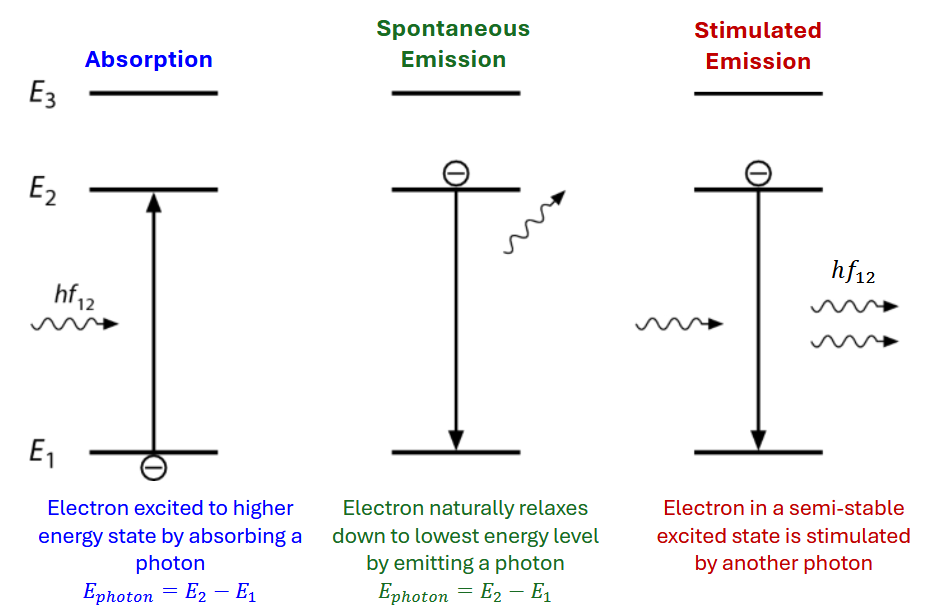
\includegraphics[width=1\textwidth]{energy transitions.png}
\end{center}
\underline{Note:} Stimulated emission occurs when an incident photon of energy equal to the energy difference between two energy levels (ex: $hf_{12}$) causes an excited electron to drop one energy level, emitting a photon of the same energy. As a result, there will be two photons of the same energy (the original photon and the emitted photon). The original photon is not absorbed but rather just causes the electron to drop energy levels.\\\\
\textbf{Lasers}\\
A key property of stimulated emission is that the emitted photon is completely in phase with the incident photon, meaning they have the same frequency, wavelength, and direction. Thus, in a three-level laser, we can create an intense beam of coherent light by using stimulated emission.\\\\
\textbf{(1)} \vspace{-2em}
\begin{center}
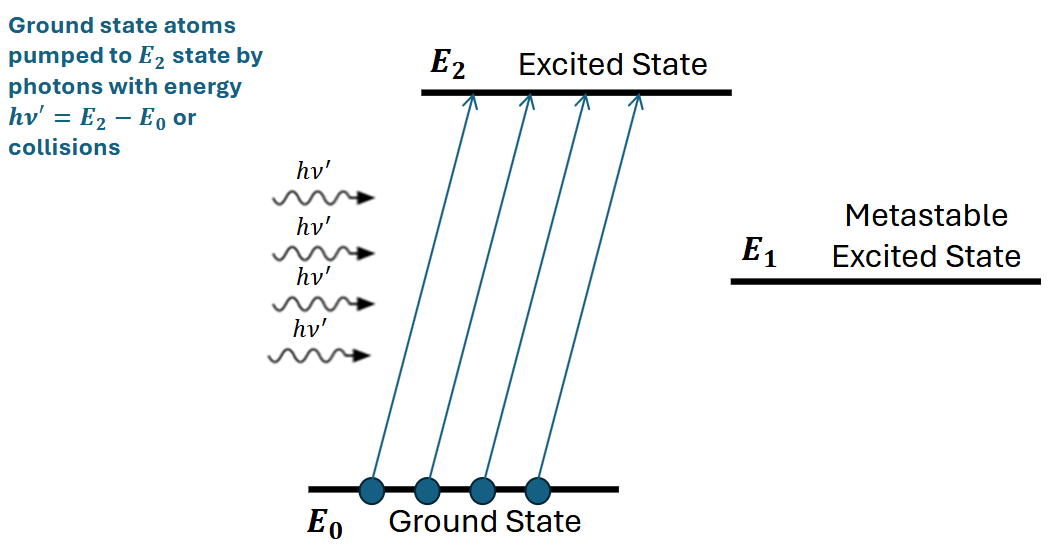
\includegraphics[width=0.6\textwidth]{laser1.png}
\end{center}
\textbf{(2)} \vspace{-2em}
\begin{center}
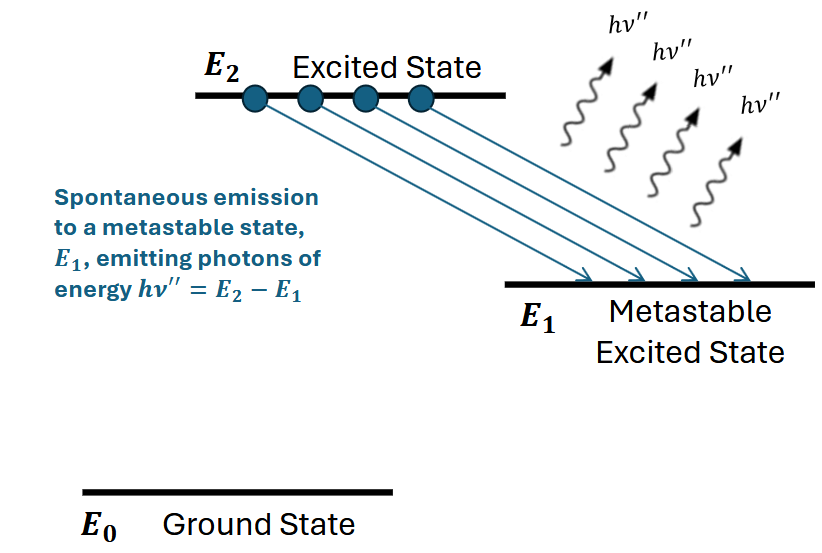
\includegraphics[width=0.6\textwidth]{laser2.png}
\end{center}
Once the electrons are at $E_1$, the metastable excited state, they can be held for long periods of time, waiting for the laser to be turned on. 
\newpage\noindent
\textbf{(3)} \vspace{-2em}
\begin{center}
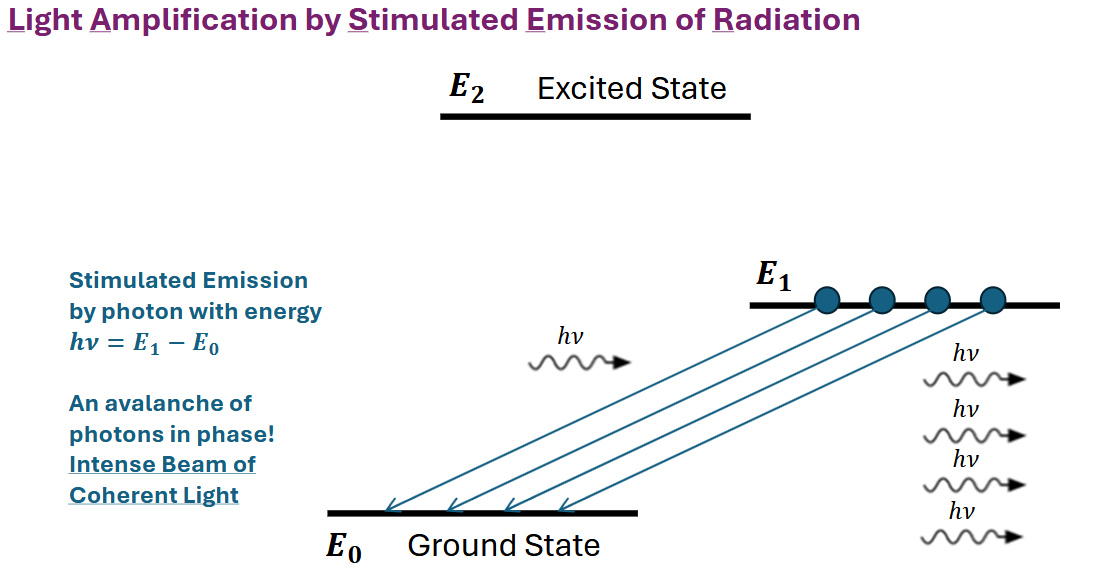
\includegraphics[width=0.6\textwidth]{laser3.png}
\end{center}
\section*{Wave-Particle Duality}
One last fundamental concept of quantum mechanics is the idea of wave-particle duality, which states that all particles exhibit both wave-like and particle-like properties.\\\\
Famously, this is demonstrated by the double-slit experiment. Interestingly, photons (and electrons) exhibit both wave-like and particle-like behaviors depending on whether they are being observed. If a detector is placed at the slits to know exactly which slit the photon goes through, then the photons will behave like particles and create two bands of light on the screen. However, if there is no detector at the slits, then the photons will behave like waves and create an interference pattern on the screen.
\begin{center}
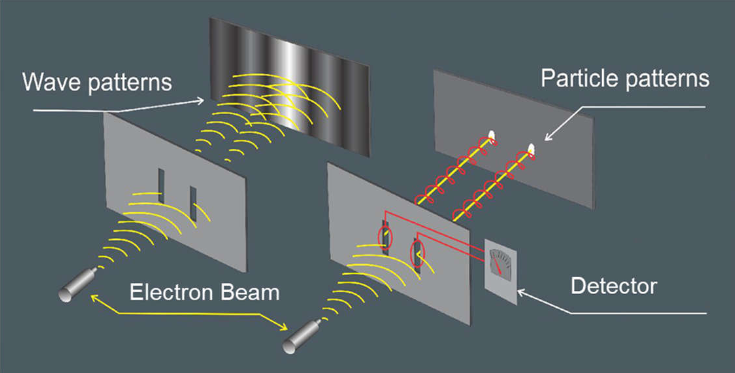
\includegraphics[width=0.8\textwidth]{double slit.png}
\end{center}
Following the experiment with electrons, we can conclude that \textit{all quantum particles} exhibit wave-particle duality, not just photons.
\newpage\noindent
\textbf{Matter Waves}\\
De Broglie proposes that if matter particles with momentum $p=mv$ exhibit wave-like properties, then they must have a wavelength given by:
\[\boxed{\lambda = \frac{h}{p}\quad\text{(De Broglie Wavelength)}}\]
\section*{Bohr Model of the Atom}
The Bohr model of the atom combines two fundamental ideas of quantum mechanics to model how electrons behave inside an atom:
\begin{itemize}
    \item \textbf{Quantized Energy (photon):} from Planck's model of blackbody radiation and Einstein's photoelectric effect, energy transitions of electrons occur in discrete amounts:
    \[E_\text{photon} = h \nu\]
    \item \textbf{Wave-Particle Duality:} De Broglie's matter waves relates an electron's wavelength to its momentum
    \[\lambda = \frac{h}{p}\]
\end{itemize}
Starting from the classical Rutherford model of the atom, let's first determine the energy of a bound electron in a circular orbit around the nucleus and its De Broglie wavelength.\\\\
\textbf{Energy of a Bound Electron}\\
In a hydrogen atom:\\\\
\begin{minipage}[t]{0.3\textwidth}
\vspace{0em}
\begin{center}
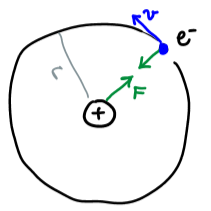
\includegraphics[width=\textwidth]{rutherford atom.png}
\end{center}
\end{minipage}
\hfill
\begin{minipage}[t]{0.6\textwidth}
\vspace{0em}
\[\sum F = m_e \vec{a}, \quad \vec{a}=\frac{v^2}{r}(-\hat{r})\quad\text{(centripetal acceleration)}\]
\[\implies \frac{q_e q_p}{4\pi\varepsilon_0 r^2}\hat{r} = \frac{-e^2}{4\pi\varepsilon_0 r^2} \hat{r}= -m_e \frac{v^2}{r}\hat{r}\]
\[\implies v = \frac{e}{\sqrt{4\pi\varepsilon_0 m_e r}}\]
\end{minipage}\\
The total energy of the hydrogen atom is the sum of the kinetic energy of the electron (assumed proton at rest) and the potential energy of the electron-proton system:
\[E_H = K+U\]
\[K = \frac{1}{2} m_e v^2 = \frac{1}{2} m_e \left(\frac{e}{\sqrt{4\pi\varepsilon_0 m_e r}}\right)^2 = \frac{e^2}{8\pi\varepsilon_0 r}\]
\[U =\frac{q_1q_2}{4\pi\varepsilon_0 r} =-\frac{e^2}{4\pi\varepsilon_0 r}\]
\[\implies \boxed{E_H = \frac{-e^2}{8\pi\varepsilon_0 r}}\]
Note that the energy of the atom depends on the radius of the electron's orbit! We will later see that this radius is quantized, which will mean energy is also quantized.\\\\
The energy is negative because the electron is bound to the nucleus, meaning it would require energy to be added to the system to free the electron from the nucleus.\\\\
\textbf{De Broglie Wavelength of the Electron}\\
Using the calculated velocity of the electron, we can find its momentum and thus its De Broglie wavelength:
\[\lambda = \frac{h}{p} = \frac{h}{m_e v}, \quad v = \frac{e}{\sqrt{4\pi\varepsilon_0 m_e r}}\]
\[\implies \boxed{\lambda = \frac{h}{e}\sqrt{\frac{4\pi\varepsilon_0r}{m_e}}}\]
Notice that the wavelength is also dependent on the radius of the electron's orbit.\\\\
\textbf{Condition for Orbital Stability}\\
So, what does it mean for an electron to have a wavelength? Recall that any bound wave must be a standing wave, because otherwise the wave would interfere with itself and cancel out. In the case of the bound electron, the standing wave must be bound to the \textit{circumference} of the electron's orbit.\\\\
\begin{minipage}[t]{0.25\textwidth}
\vspace{0em}
    \begin{center}
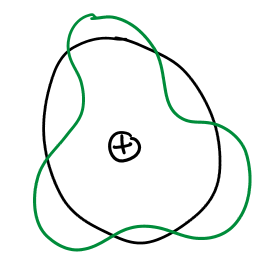
\includegraphics[width=\textwidth]{standing wave.png}
\end{center}
\end{minipage}
\hfill
\begin{minipage}[t]{0.7\textwidth}
    \vspace{0em}
Thus, the \textit{condition for orbital stability} is that the circumference of the electron's orbit must be an integer multiple of its De Broglie wavelength:
\[\boxed{2\pi r_n = n\lambda}\]
Where $n=1, 2, 3, \ldots$ is the quantum number, and $r_n$ is the radius of the electron's orbit containing $n$ wavelengths.
\end{minipage}\\
Plugging in the expression for $\lambda$, we can find the equation for the \textit{discrete radii} of the electron's orbit:
\[\boxed{r_n = \frac{n^2 h^2 \varepsilon_0}{\pi m_e e^2}}\]
For $n=1$, the radius of the electron's orbit at the ground state is called the \textbf{Bohr radius}:
\[r_1 = a_B = \frac{h^2 \varepsilon_0}{\pi m_e e^2} = 5.3 \times 10^{-11} \, \text{m}\]
Using the Bohr radius, we can simplify the equation for the discrete radii of the electron's orbit:
\[\boxed{r_n = n^2 a_B}\]
Finally, using the discrete radii, we can now find the discrete energy levels of the electron in the hydrogen atom:
\[E_n = \frac{-e^2}{8\pi\varepsilon_0 r_n} = \frac{-e^2}{8\pi\varepsilon_0 n^2 a_B}\]
\[|E_1| \equiv \frac{e^2}{8\pi\varepsilon_0 a_B} = 13.6 \, \text{eV}\quad \text{(ground state energy level)}\]
\[\implies \boxed{E_n = -\frac{|E_1|}{n^2}, \quad n=1,2,3,\ldots}\]
At:
\begin{itemize}
    \item $E_1= -13.6 \, \text{eV}$: ground state energy level
    \item $E_2, E_3, \ldots$: excited states
    \item $E_\infty = 0$: no longer bound to the nucleus (ionization)
\end{itemize}
Thus:
\begin{itemize}
    \item $|E_n|$: binding energy of the electron at the $n$th energy level (the energy required to remove the electron from its orbit)
    \item $E_1$: ionization energy (the energy required to remove the electron from the ground state, making it an ion)
\end{itemize}
\textbf{Connection to Absorption and Emission Spectra}\\
Now that we have quantized energy levels for the electron in the hydrogen atom, we can explain the discrete wavelengths of light emitted and absorbed by hydrogen.\\\\
Since the electron absorbs a photon to move up energy levels and emits a photon to move down energy levels, the transition between energy levels must be equal to the energy of the photon:
\[E_\text{photon} = hf = |E_n - E_m| \implies f_\text{photon} = \frac{|E_n-E_m|}{h}\]
\begin{center}
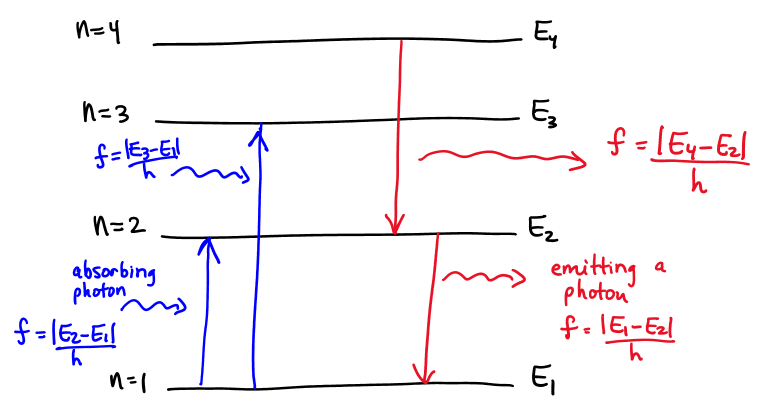
\includegraphics[width=0.6\textwidth]{discrete spectra.png}
\end{center}
Generalizing the frequency of light absorbed or emitted for a transition between $m\to n$ energy levels:
\[\boxed{f_{m\to n} = \frac{E_n-E_m}{h}=\frac{e^2}{8\pi \varepsilon_0 h a_B}\left(\frac{1}{m^2}-\frac{1}{n^2}\right)}\]
The corresponding wavelength of light absorbed or emitted is then:
\[\lambda_{m\to n} = \frac{c}{f_{m\to n}} = \frac{8\pi\varepsilon_0 h c a_B}{e^2 \left(\frac{1}{m^2}-\frac{1}{n^2}\right)}\]
\[\lambda_0 = \frac{8\pi\varepsilon_0 h c a_B}{e^2} = 91.12\, \text{nm}\]
\[\implies \boxed{\lambda_{m\to n} = \frac{\lambda_0}{(1/m^2 - 1/n^2)}\quad\text{(Balmer Formula)}}\]
Where $m=1, 2, 3, \ldots$ and $n>m$, and $\lambda_0$ is the wavelength of transition from $m=1$ to $n=\infty$.\\\\
\textbf{Angular Momentum is also Quantized}\\
Since the radius is quantized, the velocity is also quantized, which means the angular momentum of the electron is also quantized:
\[2\pi r_n = n\lambda = n\frac{h}{m_e v}\]
\[L = m_e v r_n = n\frac{h}{2\pi}\]
\[\implies \boxed{L = n\hbar, \quad \hbar = \frac{h}{2\pi}}\]
\underline{Note:} The Bohr model works only for hydrogen and hydrogen-like ions (one electron orbiting a nucleus with atomic number $Z$). We account for varying nuclei with:
\[r_n = \frac{n^2 a_B}{Z}, \quad E_n = \frac{-|E_1|Z^2}{n^2}\]
Where $|E_1|=13.6$ eV is the ground state energy level of hydrogen.
\newpage
{\centering\LARGE Unit 5: Quantum Mechanics\par}\noindent
After solidifying the core concepts of quantum mechanics in unit 4, we were able to develop more accurate models of physical phenomena, such as the Bohr model of the atom. In unit 5, we will move from these conceptual foundations to introduce the formal mathematical and probabilistic framework of quantum mechanics. Shifting from deterministic classical models to probabilistic models using the wavefunction $\psi$.
\end{document}